\documentclass[12pt]{article}
\usepackage{../eplcrypto}
\usepackage{geometry} % see geometry.pdf on how to lay out the page. There's lots.
\geometry{a4paper} % or letter or a5paper or ... etc
% \geometry{landscape} % rotated page geometry
\usepackage[parfill]{parskip}
% See the ``Article customise'' template for come common customisations
\usepackage{amsmath}
\usepackage{graphicx}
\usepackage{amssymb}
\usepackage{algorithmic}
\usepackage{algorithm}
\usepackage{tikz}

\usetikzlibrary{calc,positioning}


\title{Slides07}

%%% BEGIN DOCUMENT
\begin{document}

\maketitle
\tableofcontents
\newpage


\section{Commitment schemes}
Properties we look for:
\begin{itemize}
\item \textbf{Binding:} Once I send a value locked in a box, I cannot change it anymore.
\item \textbf{Hiding:} Nobody can tell what is inside the box, without the key.
\end{itemize}

A commitment scheme is a triple $\langle \Gen, \Com, \Open \rangle$ of PPT algorithms:
\begin{itemize}
\item $\Gen$ probabilistically selects $pk \leftarrow \Gen(1^n)$
\item $\Com$ provides $(c,d) \leftarrow \Com_{pk}(m)$
\item $\Open$ provides $m \define \Open_{pk}(c,d)$ (or $\bot$ if $c$ and $d$ do not match)
\end{itemize}
s.t., $\exists$ negl. $\negl$ : $\forall n$, $pk \leftarrow \Gen(1^n)$, and $\forall m$:
\begin{equation*}
Pr[\Open_{pk}(\Com_{pk}(m)) \neq m] < \negl(n)
\end{equation*}
Assumptions $|pk| \ge n$ and $pk$ is always generated correctly.

\subsection{Hiding property}

\subsubsection{Experiment: $\Comhide$}
Given $\Pi \define \langle \Gen, \Com, \Open \rangle$ and adversary $\A$:
\begin{enumerate}
	\item Generate $pk \leftarrow \Gen(1^n)$
	\item $\A(pk)$ outputs $m_0,m_1$
	\item Choose $b \leftarrow \bset$, compute $(c,d) \leftarrow \Com_{pk}(m_b)$ and send $c$ to $\A$
	\item $\A$ outputs $b'$
	\item Define $\Comhide(n) \define 1 \iff b=b'$ 
\end{enumerate}

$\Pi \define \langle \Gen, \Com, \Open \rangle$ is \textbf{perfectly hiding} if $\forall \A$:
\begin{equation*}
	Pr[\Comhide(n)=1] = \frac12
\end{equation*}

$\Pi \define \langle \Gen, \Com, \Open \rangle$ is \textbf{computationally hiding} if $\forall$ PPT $\A$, $\exists$ negl. $\negl$:
\begin{equation*}
	Pr[\Comhide(n)=1] \le \frac12 + \negl(n)
\end{equation*}
\newpage
\subsection{Binding property}
\subsubsection{Experiment: $\Combind$}
\begin{enumerate}
	\item Generate $pk \leftarrow \Gen(1^n)$
	\item $\A(pk)$ outputs $\langle c,d_0, d_1 \rangle$
	\item Define $\Combind(n) \define 1$ iff:
	\begin{enumerate}
		\item $\Open_{pk}(c,d_0)=m_0 \neq \bot$
		\item $\Open_{pk}(c,d_1)=m_1 \neq \bot$
		\item $m_0 \neq m_1$
	\end{enumerate}
\end{enumerate}
$\A$ provides two different openings for a commitment.\\

$\Pi \define \langle \Gen, \Com, \Open \rangle$ is \textbf{perfectly binding} if $\forall \A$:
\begin{equation*}
	Pr[\Combind(n)=1] = 0
\end{equation*}

$\Pi \define \langle \Gen, \Com, \Open \rangle$ is \textbf{computationally binding} if $\forall$ PPT $\A$, $\exists$ negl. $\negl$:
\begin{equation*}
	Pr[\Combind(n)=1] \le \negl(n)
\end{equation*}


\textbf{No commitment scheme is both perfectly binding and hiding.}\\
Intuition: In order to be perfectly hiding, it must be the case that two different messages can produce the same commitment string. But then that commitment can be opened in two ways (by an unbounded committer), so the scheme is not perfectly binding\\
Or:  If the scheme is perfectly binding, then a given commitment can only be opened on one single message m, which an unbounded adversary can find, so it cannot be perfectly hiding


\subsection{Who should choose the public key?}
\begin{itemize}
\item In the perfectly binding scheme\\
The committer: This is because the property that is computational is hiding, and if the receiver chooses the public key, then he can arrange it in such a way that this computational property is at risk. 
\item In the perfectly hiding scheme\\
The receiver: The computational property is binding here, which the committer would  want to break. It can pick pk in such a way that the committer can provide two different openings for a commitment.
\end{itemize}


\section{Zero knowledge proofs}
I want to prove that I am the one who knows this secret, without offering any other knowledge. \\
Idea: Make sure the verifier already knows my answer.
\begin{figure}[ht]
    \centering
    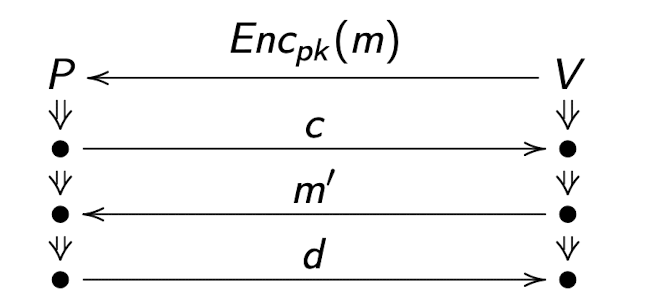
\includegraphics[width=8cm]{figures/f1.png}
\end{figure}
\begin{itemize}
\item P proves that he knows the $sk$ matching his public key p$k$
\item $(c,d) \leftarrow \Com(m)$
\item $d$ is only sent if $m=m'$
\end{itemize}

\subsection{Interactive proofs}
There ingredients:
\begin{enumerate}
\item A prover $P$, possible unbounded
\item A verifier $V$, PPT bounded
\item A language $L \subset \bset^*$ defining a set of true statements
\end{enumerate}
Motivations:
\begin{itemize}
\item Even if $P$ is unbounded, he should not be able to prove wrong things
\item $V$ must be able to perform his task efficiently
\item $L$ can be a lot of things:
	\begin{itemize}
	\item A set of DH tuples $\langle g,g^x,g^y,g^{xy} \rangle$
	\item A set of pairs of isomorphic graphs
	\item set of true theorem statements
	\end{itemize}
\end{itemize}
\newpage

The pair $P,V$ is an interactive proof system for $L$ if:
\begin{enumerate}
\item \textbf{Completeness:} If $\mathbf{x} \in L$ then the probability that P does not convince $V$ is negligible in $|\mathbf{x}|$.
\item \textbf{Soundness:} If $\mathbf{x} \notin L$ then the probability that any $P^*$ convinces $V$ is negligible in $|\mathbf{x}|$.
\end{enumerate}
Notes:
\begin{itemize}
\item Proofs are probabilistic
\item $V$ can be convinced even if $P^*$ is unbounded
\end{itemize}

Motivation:
\begin{itemize}
\item Protect the prover: The verifier should not learn anything but the fact that \xinL
\end{itemize}
Idea:
\begin{itemize}
\item Let $trans$ be the discussion between $P$ and any PPT $V^*$ on input $\mathbf{x}$.
\item It should be feasible to produce something indistinguishable from $trans$ using just the input $\mathbf{x}$.
\end{itemize}
Observations:
\begin{itemize}
\item This "simulator" can build $trans$ in any order! (so could the verifier if he tries to produce $trans$
\item No verifier can convince that a transcript is "real", he could have produced it himself!
\end{itemize}


\subsection{Definition}
$(P,V)$ is a perfect zero-knowledge interactive proof system for $L$ if $\forall$ PPT $V^*$, $\exists$ a PPT simulator $\Sim$ s.t. $\forall \varepsilon$:
\begin{equation*}
Pr[\varepsilon(trans_{P,V^*}(\mathbf{x}))=1] = Pr[\varepsilon(trans_{\Sim}(\mathbf{x}))=1]
\end{equation*}
\begin{itemize}
\item $trans_{P,V^*}(\mathbf{x})$ is the transcript of the interaction of $P$ and $V^*$ on input $\mathbf{x}$.
\item $trans_{\Sim}(\mathbf{x})$ is the output $\Sim$ on input $\mathbf{x}$.
\item $\varepsilon$ is anyone who tries to distinguish the two transcripts. (must be PPT)
\end{itemize}
Possible to define computational zero-knowledge, the probabilities can have a negligible difference.

\section{$\Sigma$-protocols}
A family of:
\begin{itemize}
\item efficient
\item 3-moves
\item honest-verifier
\end{itemize}
zero-knowledge protocols.

\subsection{Schnorr's Protocol}
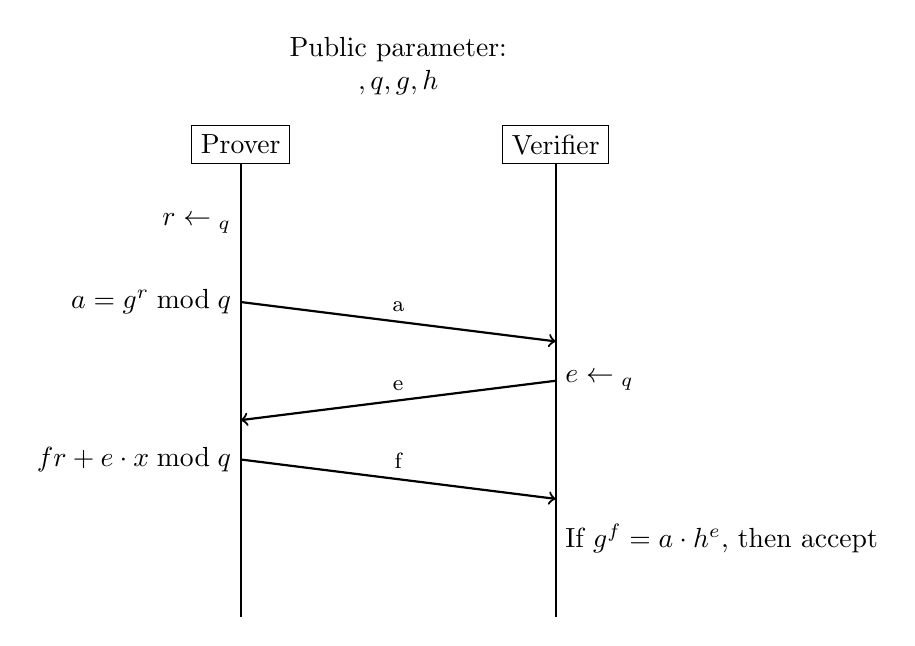
\begin{tikzpicture}
  % Public parameter:
  \node[draw=none,fill=none,align=center] (public) at (0,1) {Public parameter:\\$\GG,q,g,h$};
  % Alice
  \node[draw] (Prover) at (-2,0) {Prover}; 
  \draw[thick] (Prover) -- ++(0, -6);
    
  % Calculations of Alice
  \node[draw=none,fill=none,anchor=east] (asecret) at ($(Prover) + (0,-1)$) {$r \leftarrow {\ZZ_q}$};
  \node[draw=none,fill=none,anchor=east] (Apublic) at ($(Prover) + (0,-2)$) {$a = g^{r} \bmod{q}$};
  \node[draw=none,fill=none,anchor=east] (akey) at ($(Prover) + (0,-4)$) {$f \define r + e \cdot x \bmod{q}$};
    
  % Bob
  \node[draw] (Verifier) at (2,0) {Verifier}; 
  \draw[thick] (Verifier) -- ++(0, -6);
   
  % Calculations of Bob
  \node[draw=none,fill=none,anchor=west] (Bpublic) at ($(Verifier) + (0,-3)$) {$e \leftarrow {\ZZ_q}$};
  \node[draw=none,fill=none,anchor=west] (Bpublic) at ($(Verifier) + (0,-5)$) {If $g^f = a \cdot h^e$, then accept};
   
  % Messages
  \draw[->,thick] ($(Prover)+(0,-2)$) -- ($(Verifier)+(0,-2.5)$) node [pos=0.5,above,font=\footnotesize] {a};
  \draw[->,thick] ($(Verifier)+(0,-3)$) -- ($(Prover)+(0,-3.5)$) node [pos=0.5,above,font=\footnotesize] {e};
  \draw[->,thick] ($(Prover)+(0,-4)$) -- ($(Verifier)+(0,-4.5)$) node [pos=0.5,above,font=\footnotesize] {f};
    
\end{tikzpicture}

\textbf{(Special) Soundness:} In order to reply with non-negligible probability, $P$ must be able to respond to more than 2 challenges (with rewinding and keeping the same $a=g^r$). This actually will not happen in real life but it is to show the soundness in this protocol we think about it. Let's say $P$ replies to $e$ and $e'$. Then $\frac{g^f}{(g^x)^e} = \frac{g^{f'}}{(g^x)^{e'}}$ and $x=\frac{f-f'}{e-e'}$

\textbf{Honest verifier zero-knowledge:}
We can expect that the Verifier behaves honestly according to the specified protocol.

\newpage
\subsection{$\Pi$ is a $\Sigma$-protocol for relation $R$ if}
\begin{itemize}
\item It is a 3-move protocol with completeness, made of a $commitment$, followed by a random $challenge$, and ending with a response.
\item For any pair $(a,e,f)$ and $(a,e'.f')$ of accepting conversations on input $\mathbf{x}$ where $e \neq e'$. one can efficiently compute $\mathbf{w}:(\mathbf{x},\mathbf{w}) \in R$\\
w is the witness for statement x. like $x=g^w$
\item There is an efficient simulator that, on input $\mathbf{x},e$, produces $(a,f)$ such that $(a,e,f)$ is distributed as in a normal proof.
\end{itemize}
Not just a proof that \xinL $=\{\mathbf{x} : \exists \mathbf{w} \text{ s.t. } (\mathbf{x},\mathbf{w}) \in R \}$ but \textbf{proof of knowledge} of a witness $\mathbf{w} : (\mathbf{x},\mathbf{w}) \in R$


\subsection{Non-interactive ZK}
Let $\H$ be a random function:
\begin{itemize}
	\item Compute $e \define \H(a,\mathbf{x})$ and send non-interactive proof $(a,e,f)$
\end{itemize}

$\H$ makes sure that you pick $a,\mathbf{x}$ before seeing $e$. The only way of seeing the right $e$ is to evaluate $\H$ on $a,\mathbf{x}$.

Challenge with $\H$:
\begin{itemize}
\item We cannot use a random function. (Too big)
\item We cannot use a PRF: The prover needs to evaluate it, so he needs the key $k$, which makes it not random.
\end{itemize}


\subsubsection{The Random Oracle Model (ROM)}
\begin{itemize}
	\item Make "as if" a random function were available as an oracle for everyone.
	\item Assume that, in reality, it will work to replace it with a good hash function
\end{itemize}

Is it a sound methodology? Not really...
\begin{itemize}
	\item A real hash function has all its I/O defined in advance. A real random oracle has its I/O unknown as long as it  has not been queried.
	\item A real hash function might be computed in different ways, the output of a RO can only be known by querying the RO
\end{itemize}

But it is still used as a "not-too-bad" methodology. And good hash functions in practice give a random-looking output for any fresh input (of a given length).


\subsubsection{Strategy for $\S$ to build $trans=(a,e,f)$}
\begin{enumerate}
	\item Pick random $e$
	\item Run the $\Sigma$-protocol simulator, and get $(a,e,f)$
	\item Decide that $\H(a, \mathbf{x})=e$
\end{enumerate}
This works since: e is uniformly random, the simulator works, and $a$ is a fresh value, unlikely to have been queries to $\H$ before.

\textbf{We can transform any HVZK $\Sigma$-protocol into a NIZK protocol}. But security only holds in the ROM.

\section{Proving statements about Elgamal ciphertexts}
\begin{itemize}
\item Public key: $(g,h)\define (g,g^x)$
\item Ciphertext: $(c_1,c_2)\define (g^y,m\cdot g^{xy})$
\end{itemize}

Statement:
\begin{itemize}
\item $(c_1,c_2)$ is an encryption of $m$ under $(g,h)$
\item witness $\mathbf{w}:$ either $x$ or $y$
\end{itemize}

Reformulation:\\
L contains all $\mathbf{x} = (g_1,g_2,g_3,g_4)$ s.t. $\log_{g_1}(g_2) = \log_{g_2}(g_4)$
\begin{itemize}
\item Either $(g_1,g_2,g_3,g_4) \define (g,g^x,g^y ,g^{xy})$ (witness is $x$)
\item Either $(g_1,g_2,g_3,g_4) \define (g,g^y,g^x ,g^{xy})$ (witness is $y$)
\end{itemize}

\subsection{Chaum-Pedersen protocol}
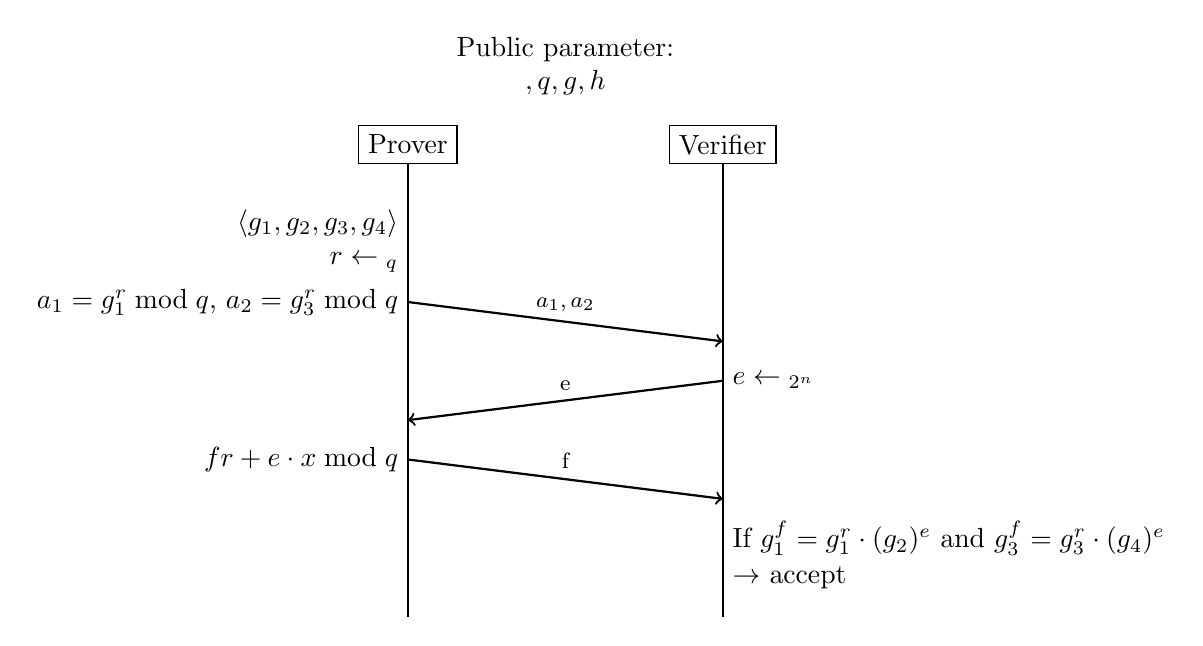
\begin{tikzpicture}
  % Public parameter:
  \node[draw=none,fill=none,align=center] (public) at (0,1) {Public parameter:\\$\GG,q,g,h$};
  % Alice
  \node[draw] (Prover) at (-2,0) {Prover}; 
  \draw[thick] (Prover) -- ++(0, -6);
    
  % Calculations of Alice
  \node[draw=none,fill=none,anchor=east] (asecret) at ($(Prover) + (0,-1)$) {$\langle g_1,g_2,g_3,g_4\rangle$};
  \node[draw=none,fill=none,anchor=east] (asecret) at ($(Prover) + (0,-1.5)$) {$r \leftarrow {\ZZ_q}$};
  \node[draw=none,fill=none,anchor=east] (Apublic) at ($(Prover) + (0,-2)$) {$a_1 = g_1^{r} \bmod{q}$, $a_2 = g_3^{r} \bmod{q}$};
  \node[draw=none,fill=none,anchor=east] (akey) at ($(Prover) + (0,-4)$) {$f \define r + e \cdot x \bmod{q}$};
    
  % Bob
  \node[draw] (Verifier) at (2,0) {Verifier}; 
  \draw[thick] (Verifier) -- ++(0, -6);
   
  % Calculations of Bob
  \node[draw=none,fill=none,anchor=west] (Bpublic) at ($(Verifier) + (0,-3)$) {$e \leftarrow {\ZZ_{2^n}}$};
  \node[draw=none,fill=none,anchor=west] (Bpublic) at ($(Verifier) + (0,-5)$) {If $g_1^f = g_1^r\cdot (g_2)^e$ and $g_3^f = g_3^r\cdot (g_4)^e$};
    \node[draw=none,fill=none,anchor=west] (Bpublic) at ($(Verifier) + (0,-5.5 )$) {$\rightarrow$ accept};
   
  % Messages
  \draw[->,thick] ($(Prover)+(0,-2)$) -- ($(Verifier)+(0,-2.5)$) node [pos=0.5,above,font=\footnotesize] {$a_1, a_2$};
  \draw[->,thick] ($(Verifier)+(0,-3)$) -- ($(Prover)+(0,-3.5)$) node [pos=0.5,above,font=\footnotesize] {e};
  \draw[->,thick] ($(Prover)+(0,-4)$) -- ($(Verifier)+(0,-4.5)$) node [pos=0.5,above,font=\footnotesize] {f};
\end{tikzpicture}

$P$ proves that $\log_{g_1}(g_2) = \log_{g_2}(g_4)$, which is the statement $x$.\\
\textbf{Soundness}: works with the same witness extractor as before. $((a_1,a_3),e,f)$ and  $((a_1,a_3),e',f')$ then $\log_{g_1}(g_2) = \log_{g_2}(g_4) = \frac{f-f'}{e-e'}$ 

\textbf{Honest verifier zero-knowledge}: Choose $e,f$ random and compute $g_1^r \define g_1^f / (g_2)^e$ and $g_3^r \define g_3^f / (g_4)^e$
\newpage


\section{The OR-proof}
Let $p$ be a prime, $q$ a prime divisor in $p-1$, and $g$ an element of order $q$ in $\ZZ_p^*$, $w \in \ZZ_q$.

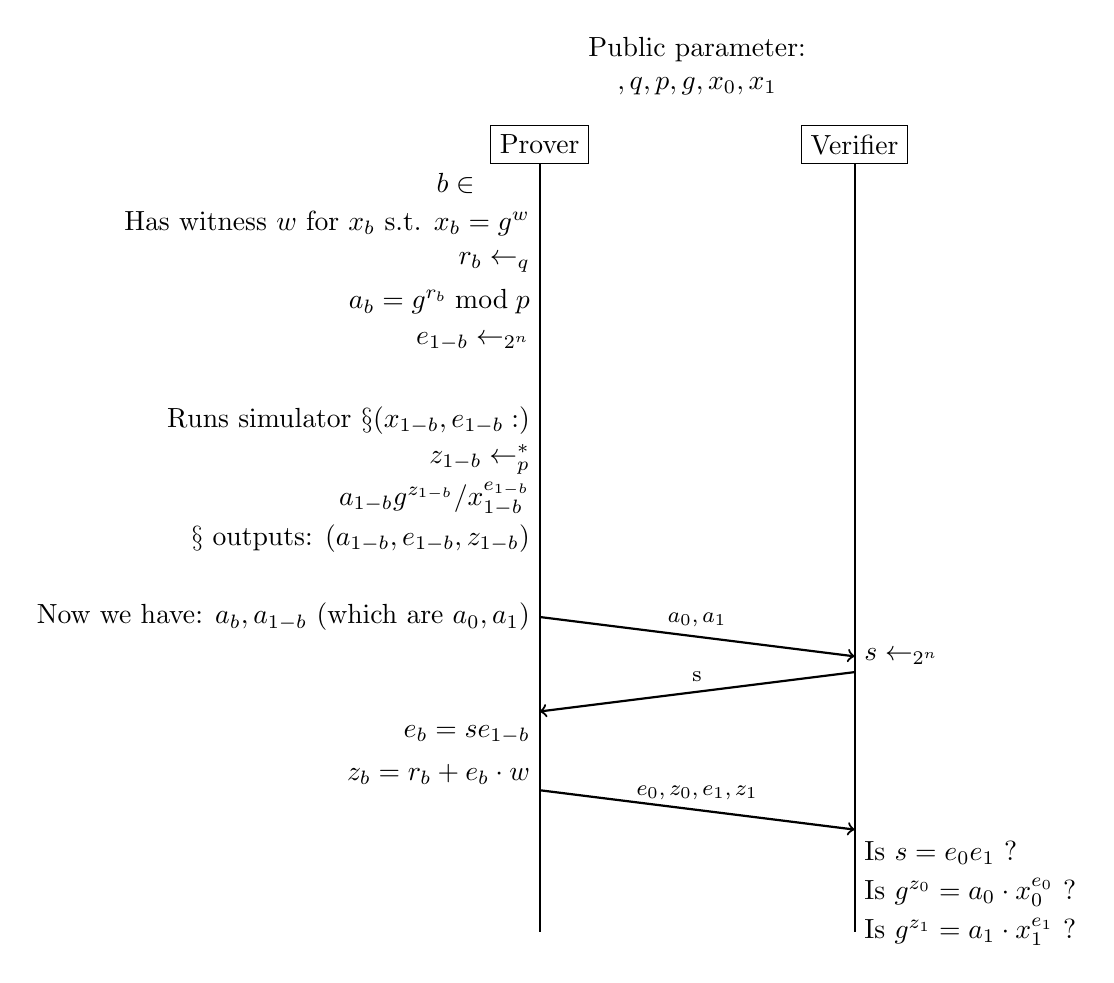
\begin{tikzpicture}
	  % Public parameter:
	  \node[draw=none,fill=none,align=center] (public) at (0,1) {Public parameter:\\$\GG,q,p,g,x_0,x_1$};
	  % Alice
	  \node[draw] (Prover) at (-2,0) {Prover}; 
	  \draw[thick] (Prover) -- ++(0, -10);
    
	  % Calculations of Alice
	  \node[draw=none,fill=none,anchor=east] (asecret) at ($(Prover) + (0,-0.5)$) {$b \in \bset \quad \quad$ };
	  \node[draw=none,fill=none,anchor=east] (asecret) at ($(Prover) + (0,-1)$) {Has witness $w$ for $x_b$ s.t. $x_b = g^w$ };
	\node[draw=none,fill=none,anchor=east] (asecret) at ($(Prover) + (0,-1.5)$) {$r_b \leftarrow \ZZ_q$ };
	 \node[draw=none,fill=none,anchor=east] (asecret) at ($(Prover) + (0,-2)$) {$a_b = g^{r_b} \bmod{p}$ };
	 \node[draw=none,fill=none,anchor=east] (asecret) at ($(Prover) + (0,-2.5)$) {$e_{1-b} \leftarrow \ZZ_{2^n}$ };
	 \node[draw=none,fill=none,anchor=east] (asecret) at ($(Prover) + (0,-3.5)$) {Runs simulator $\S(x_{1-b},e_{1-b}:)$};
	 \node[draw=none,fill=none,anchor=east] (asecret) at ($(Prover) + (0,-4)$) {$z_{1-b}\leftarrow \ZZ_p^*$};    
	 \node[draw=none,fill=none,anchor=east] (asecret) at ($(Prover) + (0,-4.5)$) {$a_{1-b} \define g^{z_{1-b}} / x_{1-b}^{e_{1-b}}$};
	 \node[draw=none,fill=none,anchor=east] (asecret) at ($(Prover) + (0,-5)$) {$\S$ outputs: $(a_{1-b}, e_{1-b},z_{1-b})$};
	 \node[draw=none,fill=none,anchor=east] (asecret) at ($(Prover) + (0,-6)$) {Now we have: $a_b, a_{1-b}$ (which are $a_0, a_1$)};	 
	 \node[draw=none,fill=none,anchor=east] (asecret) at ($(Prover) + (0,-7.5)$) {$e_b = s \xor e_{1-b}$};	 
	 \node[draw=none,fill=none,anchor=east] (asecret) at ($(Prover) + (0,-8)$) {$z_b = r_b + e_b\cdot w$};	 
	 
	 
	 
	 
  	% Bob
  	\node[draw] (Verifier) at (2,0) {Verifier}; 
  	\draw[thick] (Verifier) -- ++(0, -10);
   
 	% Calculations of Bob
	\node[draw=none,fill=none,anchor=west] (Bpublic) at ($(Verifier) + (0,-6.5)$) {$s \leftarrow \ZZ_{2^n}$};
	\node[draw=none,fill=none,anchor=west] (Bpublic) at ($(Verifier) + (0,-9)$) {Is $s = e_0 \xor e_1$ ?};
	\node[draw=none,fill=none,anchor=west] (Bpublic) at ($(Verifier) + (0,-9.5)$) { Is $g^{z_0} = a_0 \cdot x_0^{e_0}$ ?};
	\node[draw=none,fill=none,anchor=west] (Bpublic) at ($(Verifier) + (0,-10)$) { Is $g^{z_1} = a_1 \cdot x_1^{e_1}$ ?};
   
  	% Messages
  	\draw[->,thick] ($(Prover)+(0,-6)$) -- ($(Verifier)+(0,-6.5)$) node [pos=0.5,above,font=\footnotesize] {$a_0, a_1$};
	\draw[->,thick] ($(Verifier)+(0,-6.7)$) -- ($(Prover)+(0,-7.2)$) node [pos=0.5,above,font=\footnotesize] {s};
	\draw[->,thick] ($(Prover)+(0,-8.2)$) -- ($(Verifier)+(0,-8.7)$) node [pos=0.5,above,font=\footnotesize] {$e_0,z_0,e_1,z_1$};
\end{tikzpicture}

If Verifier confirms his checks, it must be that Prover either knows $w_0$ or $w_1$.






\end{document}